\documentclass{acmtrans2m}

\def\endbottomstuff{\end{figure}\gdef\permission{}}

\def\runningfoot{\def\@runningfoot{}}
\def\firstfoot{\def\@firstfoot{}}

\usepackage{url}
\usepackage{salgorithm}
\usepackage{graphicx} \graphicspath{{sorts/}}
\usepackage{fancyvrb}

%\acmVolume{V} 
%\acmNumber{N} 
%\acmYear{YY} 
%\acmMonth{M} 
\markboth{Peter Boothe}{A Simple, Useful Model of Virtual Memory} 
\title{A Simple, Useful, and Only Slightly Wrong Model of Virtual Memory}
\author{PETER BOOTHE\\
Manhattan College
}
\begin{abstract} 
We define a simple model of virtual memory in an effort to predict the number
of page faults that an algorithm will incur over the course of its lifetime.
We then use that model to analyze how many page faults we would expect to see
with two of the best-known and most well-studied sorting algorithms.  Then, we
run multiple experiments in an effort to show that the predictions of our model
match up with reality.
\end{abstract} 

\category{F.2.0}{Analysis of Algorithms and Problem Complexity}{General} 
\category{D.4.2}{Operating Systems}{Storage Management} [Virtual Memory]
\category{D.4.8}{Operating Systems}{Performance} [Modeling and Prediction]
\terms{Algorithms, Measurement, Experimentation} 
\keywords{Virtual Memory, Algorithm Analysis} 

\newcommand{\heapsort}{{\sc HeapSort}}
\newcommand{\quicksort}{{\sc QuickSort}}
\newcommand{\mergesort}{{\sc MergeSort}}
\newcommand{\NAA}{\textrm{NAA}}

\begin{document} 
\begin{bottomstuff} 
This research was supported by a summer grant from Manhattan College.\\
Author's Address: \url{peter.boothe@manhattan.edu}, or P. Boothe, Manhattan College Math and Computer Science Dept. RLC 201, 3840 Corlear Ave, Bronx, NY 10463
\end{bottomstuff} 
\maketitle 


As memory requirements begin to outstrip available memory on a machine, the
operating system will allocate virtual memory to supplement the available
physical memory.  There are several theoretical approaches to dealing with
virtual memory, but none of these methods are easily used after an algorithm is
already designed or implemented.  Even worse, some of the methods require
knowledge of available resources and the manual management of a process'
virtual memory.  In this paper we introduce a model of virtual memory that has
the benefits of being both simple and useful.  As designed, it is also slightly
incorrect, but it seems to work in practice nonetheless.  This new method
allows an algorithm designer or implementer to quickly derive how many page
faults their algorithm will incur on an input of size $n$, assuming the input
will not fit in available physical memory.  We describe the model
(Section~\ref{model}), carry out two sample analyses using the model
(Section~\ref{analysis}), and then experimentally validate the conclusions of
our analysis (Section~\ref{experiment}). 

The penalty for a page fault in virtual memory can be extreme, and can make
previously-small constants quite large. Thus, it would be of great use to be
able to easily estimate, for a given algorithm, the number of times the
algorithm will have to wait for the operating system to retrieve virtual memory
pages off the hard drive.  On a modern system, the CPU can perform 2 billion
operations a second, but the access time to retrieve a page of virtual memory
from a consumer hard drive can be multiple milliseconds.  Even if we assume
ultra-fast hard drives, a lower bound of 1 millisecond seems more than
resonable, which mean that the process is stalled, waiting for memory, for more
than 2 million wasted CPU operations.  If each tick of the CPU clock took a
second, then a virtual memory page fault would impose a penalty of more than 23
days!  Clearly, it would be good to be able to asymptotically compare the
behavior of different algorithms in the presence of virtual memory, so as to
minimize the number of page faults.

Prior work in this area is either sparse, or mind-blowingly large, depending on
whether one counts the development of cache-oblivious algorithms\cite{cacheo},
external memory sorting, and the optimization of sorting
algorithms\cite{314324,radix} as related work.  Our purpose here, however, is a
bit different.  Instead of designing an algorithm for low-memory conditions, we
seek to take existing algorithms and be able to quickly analyze their
performance when memory is scarce.


\section{The Model}
\label{model}

In the worst case, every memory access will have to go to the hard drive.
This, however, is not an informative worst-case analysis.  The worst-case page
fault predictions do not reflect the real-world behavior of virtual memory ---
they reflect a situation in which every cache access is a cache miss. Our model
avoids the worst case, and instead predicts that all non-adjacent memory
accesses have a uniform non-zero probability of causing a page fault.  Also, we
make the simplifying assumption that function calls completely clear the cache,
so all initial memory accesses after a function call have the same uniform
probability of causing a page fault.

Our method of estimating the number of page faults is therefore to count the
number of non-adjacent memory accesses.  Using this, we find that we also end
up providing a quantitative measure of ``cache friendliness'', which is a term
often used, but seldom rigorously defined.  We demonstrate our method by
comparing two classic sorting techniques: \heapsort\ and \mergesort.

Before we continue, however, we should address one obvious fault of our
model --- it is not completely correct!  In particular, if given a program that
traversed an array twice the size of available memory, our model predicts that
we will see at most 1 page fault, when in actuality there will be at least
$O(\frac{n}{2})$ page faults.  This objection is correct, as far as it goes,
and means that our model can be ``gamed'' and should only serve as a
lower-bound measure of page faults if exactness is required.  However, the
extreme simplicity of our model has great appeal, so we will conduct
experiments and see if the predictions of our (admittedly slightly wrong) model
are nonetheless useful and accurate.

\section{Using the Model to Analyze Existing Algorithms}
\label{analysis}

In this section, we use our new model to analyze already-developed algorithms.
In particular, we focus on \heapsort\ and \mergesort, because it is a folk
theorem that \heapsort\ is not ``cache friendly'' and that \mergesort\ is
``cache friendly''.  In this context, we take the term ``cache friendly'' to
mean that we would expect the number of page faults from \heapsort\ to be
higher than the number of page faults from \mergesort. If our analysis can
concretize and lend rigor to this folk theorem, then our model might be useful
in other situations as well.

\subsection{\heapsort\ Page Fault Analysis} 

Our analysis of \heapsort\ is the easiest.  The \heapsort\ algorithm, which we
take from \citeN{clrs}, is defined, with all of its supporting functions, in
Figure~\ref{fig:hsort}.  The implementation we tested is from the BSD standard
library, which is available as {\tt libbsd} on Linux.

\begin{narrowfig}{1.5in}
\begin{algorithm}
\Algorithm{HeapSort}$(array, size)$\+\\
    Build-Max-Heap$(array, size)$\\
    \For $i \gets size$ \DownTo\ $2$\+\\
        exchange $array[1] \leftrightarrow array[i]$\\
        $size \gets size - 1$\\
        Max-Heapify$(array, 1, size)$\-\\
    \Return $array$\-\\
\\
\Algorithm{Build-Max-Heap}$(array, size)$\+\\
    \For $i \gets \lfloor \frac{size}{2} \rfloor$ \DownTo\ $1$\+\\
        Max-Heapify$(array, i, size)$\-\-\\
\\
\Algorithm{Max-Heapify}$(array, i, size)$\+\\
    $l \gets 2*i$\\
    $r \gets 2*i + 1$\\
    $largest \gets i$\\
    \If $l < size$ and $array[l] > array[largest]$\+\\
            $largest \gets l$\-\\
    \If $r < size$ and $array[r] > array[largest]$\+\\
            $largest \gets r$\-\\
    \If $largest \neq i$\+\\
        exchange $array[i] \leftrightarrow array[largest]$\\
        Max-Heapify$(array, largest, size)$
\end{algorithm}

\caption{\heapsort\ pseudo code.}
\label{fig:hsort}
\end{narrowfig}

In the pseudocode of \heapsort, we note that, with the exception of the very
top of the heap, at no point do we ever access memory adjacent to the most
recently used memory location.  Therefore, we predict that the number of page
faults will be proportional to the number of memory accesses, which in the case
of \heapsort\ is proportional to its runtime of $O(n \log n)$.

\subsection{\mergesort\ Page Fault Analysis} 

The \mergesort\ algorithm we adapt from \citeN{clrs} with the memory-efficiency
improvement that, in the merge step, we only copy out the first half of the
array, and merge the second half in-place.  Our implementation may be found in
Figure~\ref{fig:msort}.  In our analysis of page faults, the only consideration
is the number and location of memory accesses, and memory accesses only occur
in the ``merge'' portion of the algorithm.

\begin{figure}
{\footnotesize
\begin{Verbatim}[numbers=left,numbersep=3pt,xleftmargin=20pt]
void mergesort(int array[], long lo, long hi)
{
    int *spare;
    int ssize;
    long sindex, hindex;
    long mid;

    // Base case
    if (lo+1 >= hi) return; 

    // Recurse on each half
    mid = (lo + hi) / 2;  
    mergesort(array, lo, mid);
    mergesort(array, mid, hi);

    // Merge
    ssize = mid-lo; // Only copy out the first half
    spare = (int *)malloc(ssize * sizeof(int));
    memcpy(spare, &(array[lo]), ssize * sizeof(int));

    sindex = 0;
    hindex = mid;
    while (sindex < ssize && hindex < hi) {
        if (spare[sindex] <= array[hindex])
            array[lo++] = spare[sindex++];
        else
            array[lo++] = array[hindex++];
    }

    while (sindex < ssize) array[lo++] = spare[sindex++];

    free(spare);
}
\end{Verbatim}
}

\caption{Our \mergesort\ implementation, in C, in its entirety.}
\label{fig:msort}
\end{figure}

In merging, the first step is to allocate a new array of size equal to half of
the passed-in array.  Then, the first half of the passed-in array is copied to
the new array.  The copying is done by accessing consecutive elements of each
array, and so once the beginning of each array has been accessed, all
subsequent memory accesses are adjacent.  Therefore, the initial step has two
non-adjacent accesses.

Subsequently, we treat the latter half of the passed-in array as one queue, and
the newly-allocated array as the second queue.  We then merge by repeatedly
removing the smaller item from the front of the two queues and overwriting an
element of the passed-in array.  Every examination requires a memory access,
but in all cases except the initial examination of the fronts of the queues,
all memory accesses occur adjacent to previous memory accesses.  Therefore, to
merge the newly-allocated array and the passed-in array requires two
non-adjacent memory accesses.  In total, each call to our \mergesort\ function
can require four non-adjacent memory accesses.

Over the whole of the algorithm, we find that the number of non-adjacent
accesses for \mergesort\ on an array of size $n$ (which we will call $\NAA(n)$)
is $$\NAA(n) = 4 + 2\NAA\left(\frac{n}{2}\right)$$ By the master theorem, we
can see that $\NAA(n) \in \Theta(n)$, and we therefore expect the number of
page faults to grow linearly with the size of the input to \mergesort.

\section{Experimental Validation of Model Conclusions} 
\label{experiment}

A model can not be experimentally verified to be correct, it can only be shown
that the available tests do not prove the model wrong.  Here, we construct a
set of tests in an attempt to disprove our model.

\begin{narrowfig}{3in}
\begin{Verbatim}[numbers=left,numbersep=3pt,xleftmargin=20pt]
#include <stdio.h>
#include <stdlib.h>

/// SORTING ALGORITHM DEFINITION GOES HERE

#define Mb (1024*1024)

int main(int argc, char **argv)
{
        int *array, i;
        long SIZE;
        SIZE = atol(argv[1])*Mb/sizeof(int);
	printf("Allocated %ld ints\n", SIZE);

        array = malloc(SIZE*sizeof(int));
        fprintf(stderr, "%p\n", array);
        
        for (i = 0; i < SIZE; i++) {
            array[i] = i*7 % SIZE;
        }

        /// CALL TO SORTING ALGORITHM GOES HERE

        free(array);

        return 0;
}
\end{Verbatim}
\caption{Our test harness for both algorithms}
\label{fig:harness}
\end{narrowfig}
\subsection{Experimental Setup}

To analyze the number of major page faults in an algorithm, we must run our
algorithm in low-memory conditions so that the operating system is forced to
allocate and use virtual memory for our program.  Unfortunately, accessing swap
is incredibly slow --- a major part of the motivation for our study --- which
means that under low-memory conditions our tests may require 1000000 times more
time to finish than they would if we weren't using swap.  

We reconcile the opposing forces of our desire for speed and our desire to use
swap by running our tests in a virtual machine via the Qemu emulator.  The
machine running the emulator had 4 gigabytes of memory.  Of those 4 gigabytes,
half was allocated as a RAM disk.  The swap partition of the emulated machine
was a file stored on that RAM disk.  This meant that the page faults of the
emulated machine would still be recorded, but that the emulated machine would
not suffer a performance hit, as the emulated swap was backed by a (very fast)
RAM disk.  This technique is recommended for anyone who would like to count
page faults but does not want to waste a lot of time to do so.

Interestingly, the RAM disk turned out to be helpful, but not essential. The
natural caching behaviour of the host operating system meant that even when the
emulated swap was backed by a file on a physical hard drive, it was often
cached in the memory of the host operating system due to the host operating
system's automatic buffering of hard drive reads and writes.

\subsection{Implementations and Test Harness}

For \heapsort\ we used the implementation found in the BSD standard library,
which is available as {\tt libbsd} on Linux.  For \mergesort\ we wrote our own
implementation, which can be found in Figure~\ref{fig:msort}.  The test harness
that we used was exactly the same for both algorithms, and can be seen in
Figure~\ref{fig:harness}.  To test our algorithms, we declared and allocated a
single large array, and then we filled that array with many increasing
sequences.


\subsection{Number of Page Faults Compared}

We compare the page faults of \heapsort\ and \mergesort\ for a wide range of memory sizes and problem sizes.  We find that, for problems which do not fit into available memory, \heapsort\ incurs more page faults than \mergesort.  Holding available memory constant, in Figure~\ref{fig:sizes} we see that \mergesort\ almost always has fewer page faults than \heapsort.  We grew available memory in the virtual machine, in increments of 64 megabytes, from a low of 64 megabytes to a high of 512 megabytes.  Each line in the figure represents the behavior with a fixed amount of available memory.

\begin{figure}
\input{sorts/memsizes.tex}
\caption{Number of major page faults for \mergesort\ and \heapsort\ at a variety of memory sizes.  Note that at almost all memory sizes, \mergesort\ is better.}
\label{fig:sizes}
\end{figure}

As the ratio of problem size to available memory grows, so does the advantage
of \mergesort\ over \heapsort.  In Figure~\ref{fig:ratio}, we can see the
number of page faults of \heapsort\ divided by the number of page faults of
\mergesort\ for a variety of problem sizes.  The ratio, as predicted, rises as
the amount of memory pressure rises.  As problem sizes increase, \heapsort\
performs increasingly worse compared to \mergesort. This experimental result is
precisely in line with the results of our model which suggest that the number of page faults for \heapsort\ is asymptotically greater than the number of page faults in \mergesort\ ($O(n \log n)$ instead of $O(n)$).

\begin{figure}
% GNUPLOT: LaTeX picture with Postscript
\begingroup
  \makeatletter
  \providecommand\color[2][]{%
    \GenericError{(gnuplot) \space\space\space\@spaces}{%
      Package color not loaded in conjunction with
      terminal option `colourtext'%
    }{See the gnuplot documentation for explanation.%
    }{Either use 'blacktext' in gnuplot or load the package
      color.sty in LaTeX.}%
    \renewcommand\color[2][]{}%
  }%
  \providecommand\includegraphics[2][]{%
    \GenericError{(gnuplot) \space\space\space\@spaces}{%
      Package graphicx or graphics not loaded%
    }{See the gnuplot documentation for explanation.%
    }{The gnuplot epslatex terminal needs graphicx.sty or graphics.sty.}%
    \renewcommand\includegraphics[2][]{}%
  }%
  \providecommand\rotatebox[2]{#2}%
  \@ifundefined{ifGPcolor}{%
    \newif\ifGPcolor
    \GPcolorfalse
  }{}%
  \@ifundefined{ifGPblacktext}{%
    \newif\ifGPblacktext
    \GPblacktexttrue
  }{}%
  % define a \g@addto@macro without @ in the name:
  \let\gplgaddtomacro\g@addto@macro
  % define empty templates for all commands taking text:
  \gdef\gplbacktext{}%
  \gdef\gplfronttext{}%
  \makeatother
  \ifGPblacktext
    % no textcolor at all
    \def\colorrgb#1{}%
    \def\colorgray#1{}%
  \else
    % gray or color?
    \ifGPcolor
      \def\colorrgb#1{\color[rgb]{#1}}%
      \def\colorgray#1{\color[gray]{#1}}%
      \expandafter\def\csname LTw\endcsname{\color{white}}%
      \expandafter\def\csname LTb\endcsname{\color{black}}%
      \expandafter\def\csname LTa\endcsname{\color{black}}%
      \expandafter\def\csname LT0\endcsname{\color[rgb]{1,0,0}}%
      \expandafter\def\csname LT1\endcsname{\color[rgb]{0,1,0}}%
      \expandafter\def\csname LT2\endcsname{\color[rgb]{0,0,1}}%
      \expandafter\def\csname LT3\endcsname{\color[rgb]{1,0,1}}%
      \expandafter\def\csname LT4\endcsname{\color[rgb]{0,1,1}}%
      \expandafter\def\csname LT5\endcsname{\color[rgb]{1,1,0}}%
      \expandafter\def\csname LT6\endcsname{\color[rgb]{0,0,0}}%
      \expandafter\def\csname LT7\endcsname{\color[rgb]{1,0.3,0}}%
      \expandafter\def\csname LT8\endcsname{\color[rgb]{0.5,0.5,0.5}}%
    \else
      % gray
      \def\colorrgb#1{\color{black}}%
      \def\colorgray#1{\color[gray]{#1}}%
      \expandafter\def\csname LTw\endcsname{\color{white}}%
      \expandafter\def\csname LTb\endcsname{\color{black}}%
      \expandafter\def\csname LTa\endcsname{\color{black}}%
      \expandafter\def\csname LT0\endcsname{\color{black}}%
      \expandafter\def\csname LT1\endcsname{\color{black}}%
      \expandafter\def\csname LT2\endcsname{\color{black}}%
      \expandafter\def\csname LT3\endcsname{\color{black}}%
      \expandafter\def\csname LT4\endcsname{\color{black}}%
      \expandafter\def\csname LT5\endcsname{\color{black}}%
      \expandafter\def\csname LT6\endcsname{\color{black}}%
      \expandafter\def\csname LT7\endcsname{\color{black}}%
      \expandafter\def\csname LT8\endcsname{\color{black}}%
    \fi
  \fi
  \setlength{\unitlength}{0.0500bp}%
  \begin{picture}(7200.00,5040.00)%
    \gplgaddtomacro\gplbacktext{%
      \csname LTb\endcsname%
      \put(1078,704){\makebox(0,0)[r]{\strut{} 0}}%
      \csname LTb\endcsname%
      \put(1078,1568){\makebox(0,0)[r]{\strut{} 5}}%
      \csname LTb\endcsname%
      \put(1078,2432){\makebox(0,0)[r]{\strut{} 10}}%
      \csname LTb\endcsname%
      \put(1078,3296){\makebox(0,0)[r]{\strut{} 15}}%
      \csname LTb\endcsname%
      \put(1078,4160){\makebox(0,0)[r]{\strut{} 20}}%
      \csname LTb\endcsname%
      \put(1210,484){\makebox(0,0){\strut{} 0}}%
      \csname LTb\endcsname%
      \put(1725,484){\makebox(0,0){\strut{} 100}}%
      \csname LTb\endcsname%
      \put(2239,484){\makebox(0,0){\strut{} 200}}%
      \csname LTb\endcsname%
      \put(2754,484){\makebox(0,0){\strut{} 300}}%
      \csname LTb\endcsname%
      \put(3268,484){\makebox(0,0){\strut{} 400}}%
      \csname LTb\endcsname%
      \put(3783,484){\makebox(0,0){\strut{} 500}}%
      \csname LTb\endcsname%
      \put(4297,484){\makebox(0,0){\strut{} 600}}%
      \csname LTb\endcsname%
      \put(4812,484){\makebox(0,0){\strut{} 700}}%
      \csname LTb\endcsname%
      \put(5326,484){\makebox(0,0){\strut{} 800}}%
      \csname LTb\endcsname%
      \put(5841,484){\makebox(0,0){\strut{} 900}}%
      \csname LTb\endcsname%
      \put(6355,484){\makebox(0,0){\strut{} 1000}}%
      \csname LTb\endcsname%
      \put(6870,484){\makebox(0,0){\strut{} 1100}}%
      \put(440,2432){\rotatebox{90}{\makebox(0,0){\strut{}Ratio of Heapsort page faults to Mergesort page faults}}}%
      \put(4040,154){\makebox(0,0){\strut{}Problem size in megabytes}}%
      \put(4040,4710){\makebox(0,0){\strut{}Heapsort is bad and gets worse as problems grow}}%
      \put(4040,4490){\makebox(0,0){\strut{}Each line holds available memory constant}}%
    }%
    \gplgaddtomacro\gplfronttext{%
    }%
    \gplbacktext
    \put(0,0){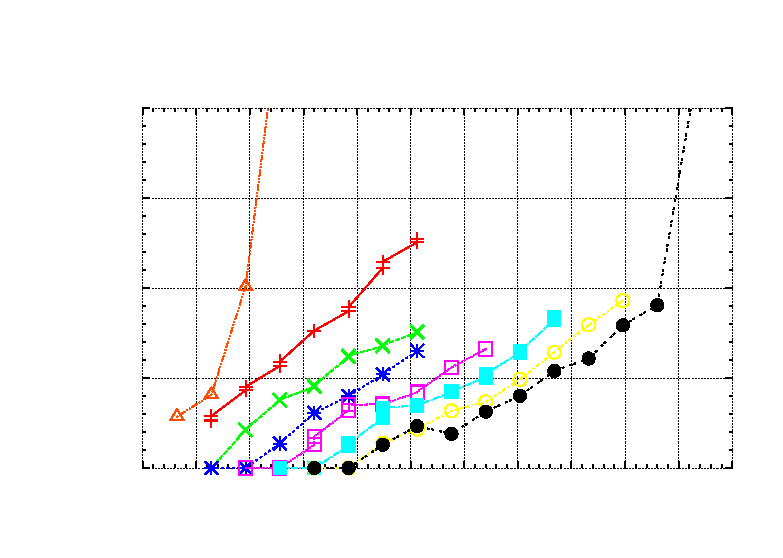
\includegraphics{ratios}}%
    \gplfronttext
  \end{picture}%
\endgroup

\caption{Number major page faults for \heapsort\ divided by the number of major page faults for \mergesort\ at a variety of memory sizes.  The fact that this ratio grows over time indicates the \heapsort\ has asymptotically more page faults than \mergesort, which is exactly what is predicted by our model.}
\label{fig:ratio}
\end{figure}

Because our experimental conclusions are in line with the conclusions of our
model, we must consider this to be evidence in favor of the model's utility.
Our experiments have failed to disprove our model, which means that it still
may be correct enough for our purposes.

\section{Conclusion}

We have described a new model of virtual memory which has the virtue of extreme
simplicity.  In this model, every memory access which is not adjacent to a previous memory access has a uniform probability of incurring a virtual memory page fault.  Furthermore, all function calls are considered to wipe out our caches, and so all memory accesses after a function call, even if adjacent to memory accessed before the function call, have that same uniform probability of causing a page fault.  This model is, as stated, extremely simple (and a bit simplistic).

In exchange for this simplicity, we had to sacrifice formal correctness.  Using
experimental techniques, we validated the utility of our method, and showed
that it does appear to be useful, and at least model the cases of \heapsort\
and \mergesort\ well.  Much like a buggy program that still remains useful for
some tasks, we find that our slightly-incorrect analysis technique can, with
relative ease, provide useful estimates regarding the asymptotic behavior of
algorithms in the presence of virtual memory.

Future work in this domain would involve testing more algorithms under adverse
memory conditions to see whether our model accurately reflects the behavior of
more algorithms than just the two tested here.  Also, a deeper understanding of
why our incorrect model gives such good and useful results (and when it can be
counted upon to do so) would be of great interest.

\bibliographystyle{acmtrans}
\bibliography{bibliography}

\begin{received} 
Submission to ALENEX 2011
\end{received}
\end{document}
